\documentclass[12pt]{article}
\usepackage{graphicx}
\usepackage[left=3cm,top=3cm,right=3cm,bottom=3cm]{geometry}

\begin{document}

\title{Bayesian evolutionary analysis of viruses:\\ A practical introduction to BEAST }

\author{Andrew Rambaut and Alexei J Drummond}

\date{\today{}}

\maketitle

\section*{Introduction}

This practical will introduce the BEAST software for Bayesian evolutionary analysis, with a focus on virus evolution. It is divided into three sections or exercises:

\begin{enumerate}
\item Rates and dates - The first exercise will take you through the process of estimating divergence times in a phylogeny when you have calibration information from fossil evidence or other prior knowledge. It will also demonstrate how to analyze a data set using a relaxed molecular clock.
\item Time-stamped data - The second exercise will demonstrate how to use BEAST to estimate the rate of evolution of a virus that has been sampled from multiple time points.
\item Bayesian skyline plot - The third exercise will take you though the estimation of population history of a virus epidemic using the Bayesian skyline plot.
\end{enumerate}

To undertake the exercises in this practical, you will need to have access to the following software packages in a format that is compatible with your
computer system (all three are available for Mac OS X, Windows and Linux/UNIX operating systems):

\begin{itemize}

\item {\bf BEAST} - this package contains the BEAST program, BEAUti, TreeAnnotator and other utility programs. At the time of writing, the
current version is v1.5.1. It is available for download from \texttt{http://beast.bio.ed.ac.uk/} and \texttt{http://code.google.com/p/beast-mcmc/downloads/list}.
\item {\bf Tracer} - this program is used to explore the output of BEAST (and other Bayesian MCMC programs). It graphically and
quantitively summarizes the distributions of continuous parameters and provides diagnostic information. At the time of
writing, the current version is v1.4.1. It is available for download from \texttt{http://beast.bio.ed.ac.uk/}.
\item {\bf FigTree} - this is an application for displaying and printing molecular phylogenies, in particular those obtained using
BEAST. At the time of writing, the current version is v1.2.3. It is available for download from \texttt{http://tree.bio.ed.ac.uk/}.
\end{itemize}

%%%%%%%%%%%%%%%%%%%%%%%%%%%%%%%%%%%%%%%%%%%%%
%%%
%%% EXERCISE 1 - RATES AND DATES
%%%
%%%%%%%%%%%%%%%%%%%%%%%%%%%%%%%%%%%%%%%%%%%%%

\section*{Exercise 1: Rates and dates}

This exercise will guide you through the analysis of an alignment of feline papilloma virus (FPV) sequences. The goal is to estimate the rate of evolution on each lineage based on dates of divergence of their host species. BEAST is currently unique in its ability to estimate
the phylogenetic tree and the divergence times simultaneously. 

The first step will be to convert a NEXUS file with a DATA or CHARACTERS block into a BEAST XML input file. This is done using the program BEAUti (this stands for Bayesian Evolutionary Analysis Utility). This is a user-friendly program for setting the evolutionary model and options for the MCMC analysis. The second step is to actually run BEAST using the input file that
contains the data, model and settings. The final step is to explore the output of BEAST in order to diagnose problems and to summarize the results.

\subsection*{BEAUti }

The program BEAUti is a user-friendly program for setting the
model parameters for BEAST. Run BEAUti by double clicking on its icon. 

\subsubsection*{Loading the NEXUS file }

To load a NEXUS format alignment, simply select the \texttt{Import
Alignment...} option from the File menu: 

\medskip{}

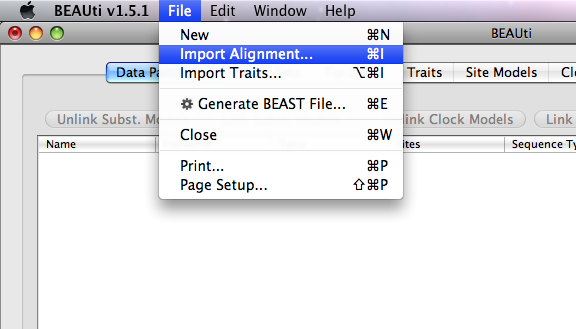
\includegraphics[scale=0.5]{figures1/ImportNexus}

\medskip{}

Select the file called \texttt{FPV.nex}. This file contains an alignment
of partial genome sequences of papilloma virus from 5 species of cat
along with related viruses from a racoon and a dog. It looks like
this (the lines have been truncated):

\begin{verbatim}
#NEXUS 

Begin data;
    Dimensions ntax=7 nchar=1434;
    Format datatype=nucleotide gap=-;
    Matrix 
CanineOralPV   ATGGCAAGGAAAAGACGCGCAGCCCCTCAAGATATATACCCTGCTTGTAAA
FelisPV1       ATGCTTAGGCAAAAACGTGCAGCCCCAAAAGATATTTACCCACAATGCAAG
LynxPV1        ATGCTACGGCGAAAACGTGCAGCCCCCCATGATATCTACCCCCAATGCAAA
PumaPV1        ATGCTTAGGCGAAAACGTGCAGCCCCCAAAGATATTTACCCCCAATGCAAA
RacoonPV1      ATGACTCGCAAACGCCGCGCCGCTCCTCGTGATATATACCCCTCTTGCAAA
AsianLionPV1   ATGCTAAGGCGAAAACGTGCAGCCCCCTCAGATATCTACCCCCAATGCAAA
SnowLeopardPV1 ATGCTAAGGCGAAAACGTGCAGCCCCTTCTGATATTTACCCACAATGCAAA
    ; 
End;
\end{verbatim}

\medskip{}

Once loaded, the list of taxa and the actual alignment will be displayed
in the main panel:

\medskip{}

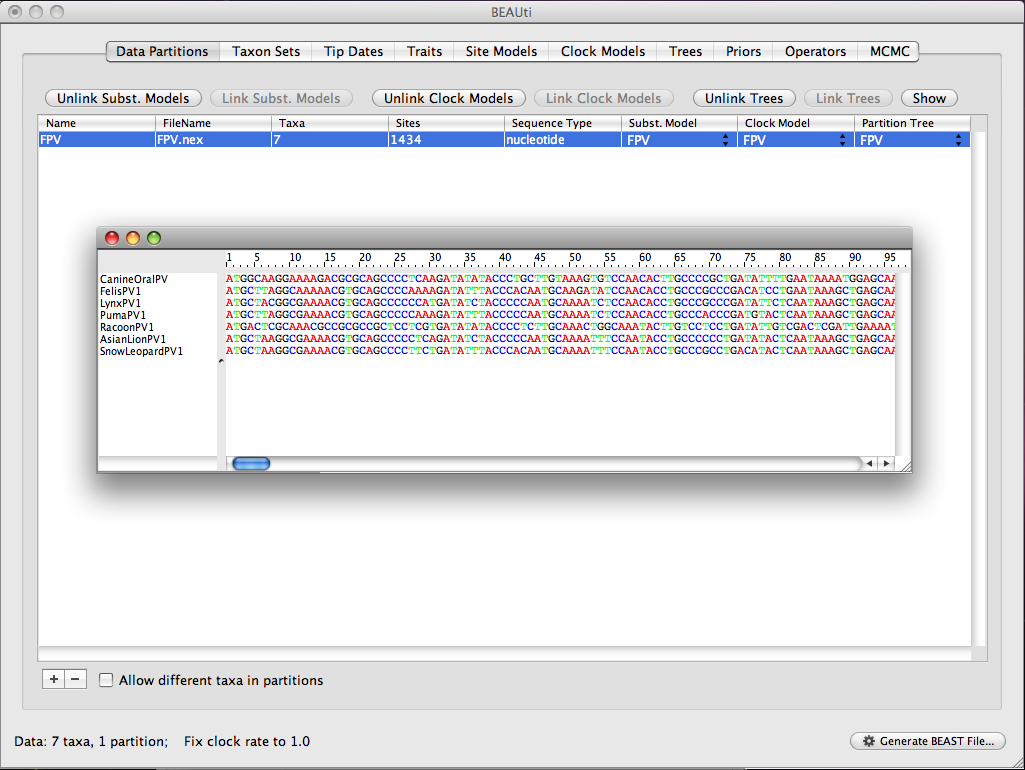
\includegraphics[scale=0.4]{figures1/BEAUti_Data}

\medskip{}

\subsubsection*{Defining the calibration nodes}

Select the {\bf Taxon Sets} tab at the top of the main window. You will see the
panel that allows you to create sets of taxa. Once you have created a taxa set you will be able to add calibration information for it most recent common
ancestor (MRCA) later on. Press the small ``plus''
button at the bottom left of the panel. This will create a new taxon
set. Rename it by double-clicking on the entry that appears (it will
initially be called \texttt{untitled1}). Call it \texttt{Felis/Lynx/Puma}.
In the next table along you will see the available taxa. Select the
\texttt{FelisPV1}, \texttt{LynxPV1} and \texttt{PumaPV1} taxa and
press the green arrow button to move them into the included taxa set.

Now repeat the whole procedure creating a set called \texttt{Lion/Leopard}
that contains on the \texttt{SnowLeopardPV1} and \texttt{AsianLionPV1}
taxa. The screen should look like this:

\medskip{}

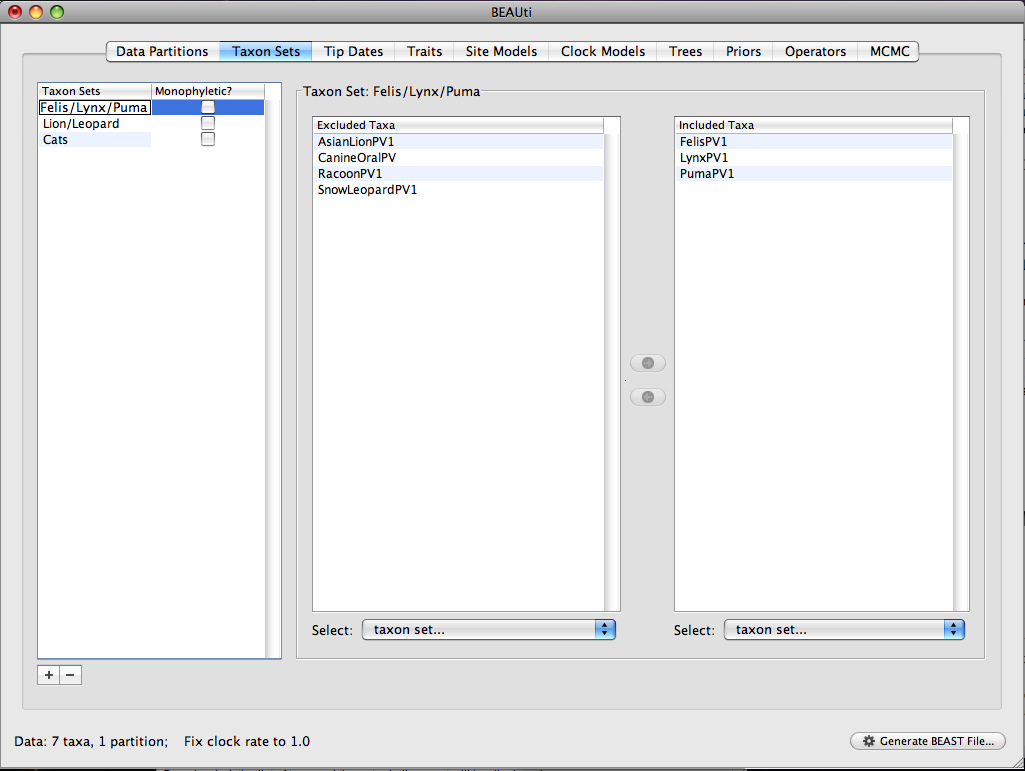
\includegraphics[scale=0.4]{figures1/BEAUti_Taxa}

\medskip{}

Finally, create a taxon group that contains all the cat papilloma
virus sequences (i.e. everything except \texttt{RacoonPV1} and \texttt{CanineOralPV}).
Call this taxon set \texttt{Cats}. If we wished to enforce the racoon
and canine PV sequences as an outgroup, we could select the checkbox
in the {\bf Monophyletic?} column. This will ensure that the \texttt{Cats}
ingroup is kept monophyletic during the MCMC analysis.
However, for this analysis we are not going to enforce this assumption
as we want to confirm that the papilloma virus' tree
is the same as the hosts'.

\subsubsection*{Setting the substitution model}

The next thing to do is to click on the {\bf Site Models} tab at the top of the
main window. This will reveal the evolutionary model settings for
BEAST. Exactly which options appear depend on whether the data are
nucleotides or amino acids.
The settings that will appear after loading the FPV data set will
be the default values so we need to make some changes. 

Most of the models should be familiar to you. For this analysis, we
will make three changes. First, select \textbf{Empirical} under the \textbf{Base
frequencies} menu. Second, select \textbf{Gamma} under the \textbf{Site
Heterogeneity Model} menu which will allow rate variation between
sites in the alignment. 

\medskip{}

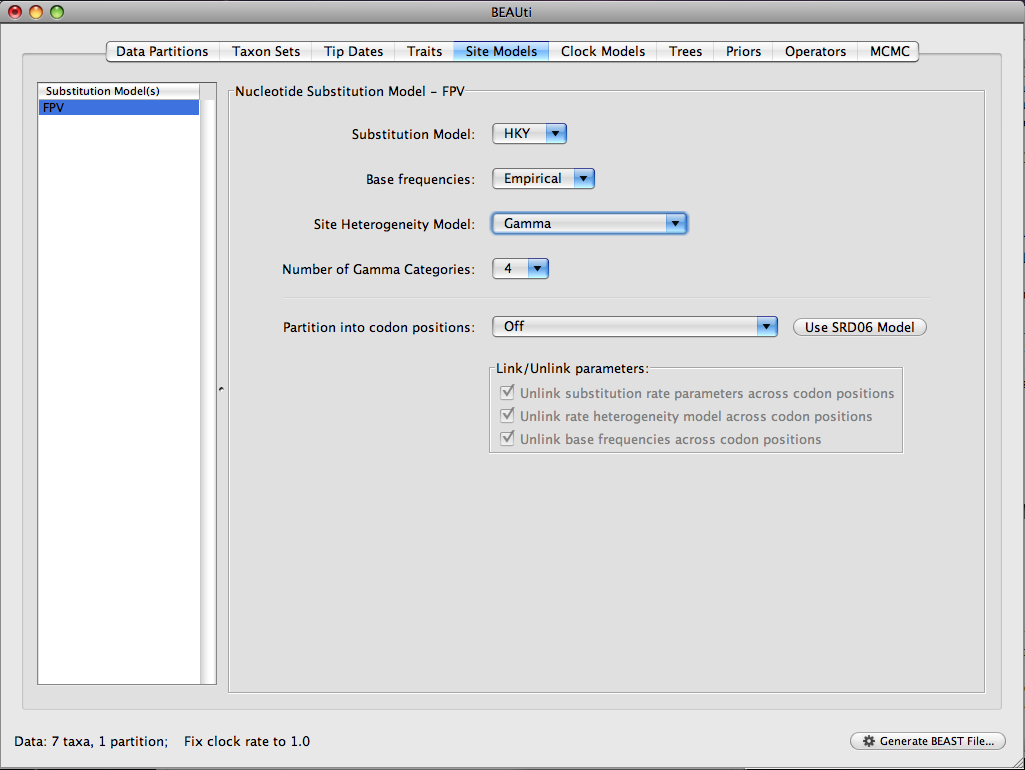
\includegraphics[scale=0.4]{figures1/BEAUti_Subst_Model}

\medskip{}

\subsubsection*{Setting the clock model}

The third thing we will do is to click on the {\bf Clock Models} tab at the top of the
main window, and to change the molecular clock model to \textbf{Relaxed Clock: Uncorrelated
Log-normal} so as to account for lineage-specific rate heterogeneity.
Your model options should now look like this: 

\medskip{}

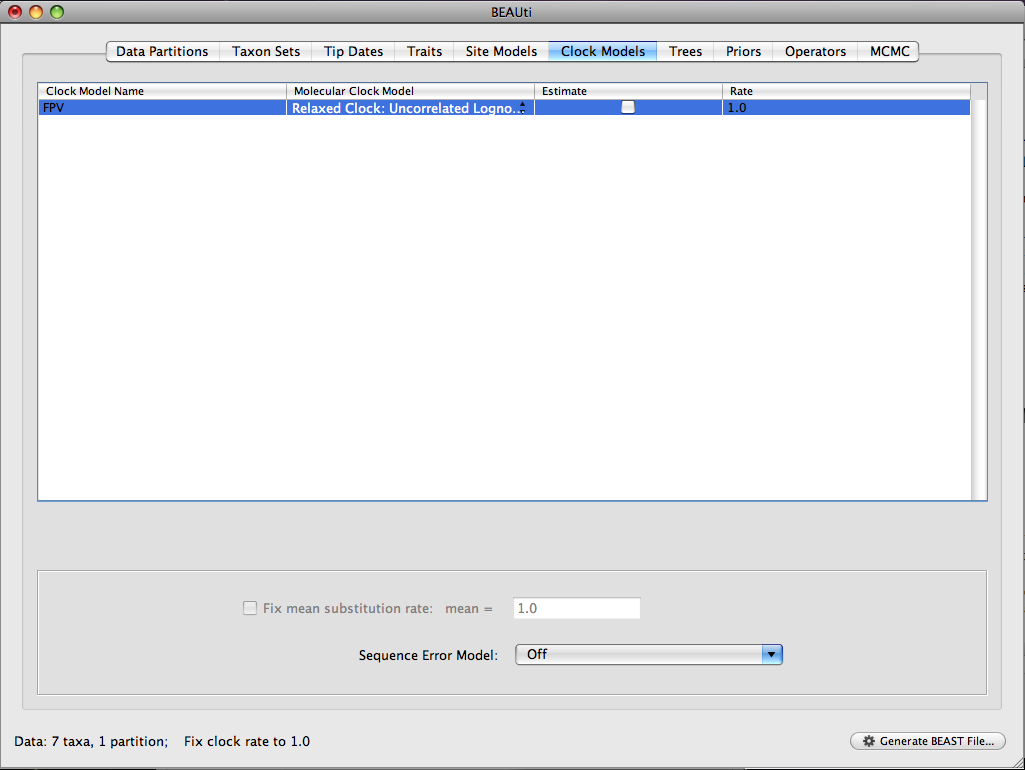
\includegraphics[scale=0.4]{figures1/BEAUti_Clock_Model}

\medskip{}

The \textbf{Estimate} check box is required to be checked. This is because we wish to estimate
the clock rate (and in doing so the divergence times). But this will be automatically checked, in this case, when we put a proper prior on \textbf{tmcra} statistics appeared in \textbf{Priors} panel.

\subsubsection*{Trees }

The {\bf Trees} tab allows priors to be specified for each parameter in the
model. The first thing to do is to specify that we wish to use the Yule model 
as the tree prior. This is a simple model of speciation that
is generally more appropriate when considering sequences from different species.
Select this from the {\bf Tree prior} dropdown menu.

\medskip{}

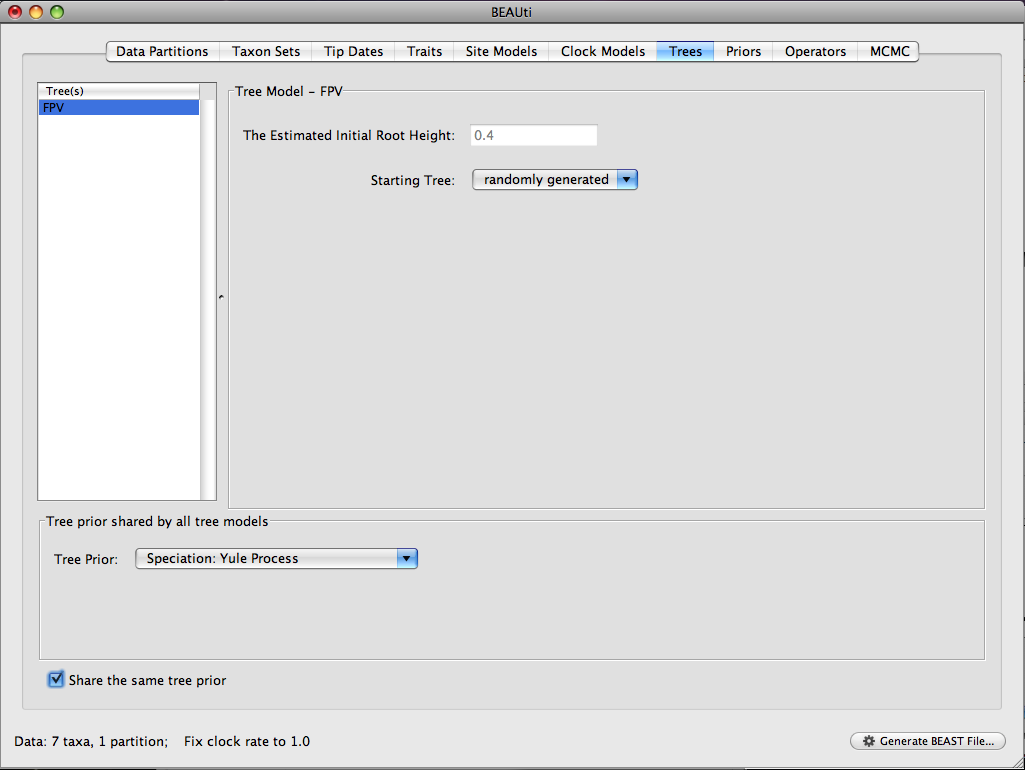
\includegraphics[scale=0.4]{figures1/BEAUti_Tree}

\medskip{}

\subsubsection*{Priors }

We now need to specify a prior distribution for some of the divergence times on {\bf Prior} panel, based on our prior fossil knowledge. This is known as calibrating our tree. We will actually use two calibrations
in this analysis. Click on the button in the table next to \texttt{tmrca(Felis/Lynx/Puma)}: 

A dialog box will appear allowing you to specify a prior for the
MRCA of these three species. Select the \textbf{Normal} distribution

\medskip{}

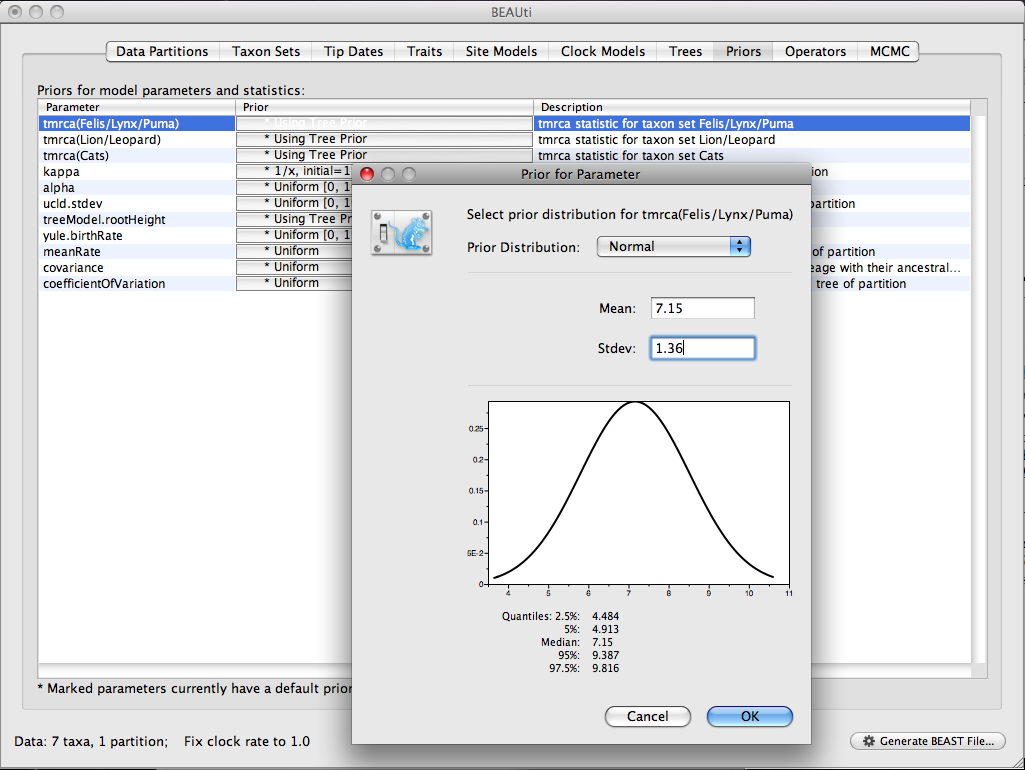
\includegraphics[scale=0.4]{figures1/BEAUti_Prior1}

\medskip{}

We are going to assume a normal distribution centered at 7.15 million
years with a standard deviation of 1.36 million years. This will give
a central 95\% range of about 4.5-9.8 My. This corresponds to the
estimate of the date of the most recent common ancestor of the host
species (\emph{Felis catus,} \emph{Puma concolor} and \emph{Lynx rufus})
reported by Rector et al. (2007). 

Following the same procedure set a calibration of 3.72 +/- 1.05 million years for the lion-leopard split. 

Although we created a taxon set for the whole cat group (\texttt{tmrca(Cats)}
in the prior table), we are not going to put an informative prior
on this. We can then compare this divergence date with that estimated
for the hosts. The priors table should now look like this: 

\medskip{}

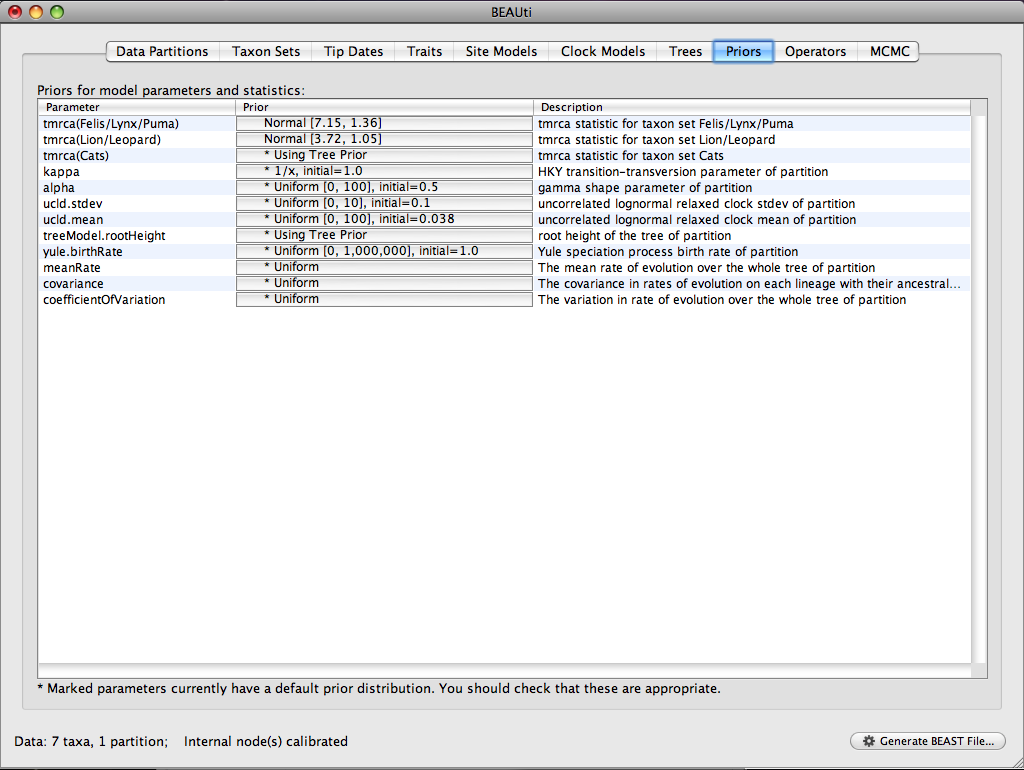
\includegraphics[scale=0.4]{figures1/BEAUti_Prior2}

\medskip{}

\subsubsection*{Setting the MCMC options }

Ignore the \textbf{Operators} tab as this just contains technical
settings effecting the efficiency of the MCMC program (see Notes for details). 

The next tab, {\bf MCMC}, provides more general
settings to control the length of the MCMC and the file names. 

Firstly we have the \textbf{Length of chain}. This is the number of
steps the MCMC will make in the chain before finishing. How long this
should be depends on the size of the data set, the complexity of the
model and the quality of answer required. The default value of 10,000,000
is entirely arbitrary and should be adjusted according to the size
of your data set. For this data set let's initially set the chain
length to 800,000 as this will run reasonably quickly on most modern
computers (a few minutes).

The next options specify how often the parameter values in the Markov
chain should be displayed on the screen and recorded in the log file.
The screen output is simply for monitoring the programs progress so
can be set to any value (although if set too small, the sheer quantity
of information being displayed on the screen will actually slow the
program down). For the log file, the value should be set relative
to the total length of the chain. Sampling too often will result in
very large files with little extra benefit in terms of the precision
of the analysis. Sample too infrequently and the log file will not
contain much information about the distributions of the parameters. 
You probably want to aim to store no more than 10,000 samples so this should be
set to no less than chain length / 10,000.

\medskip{}

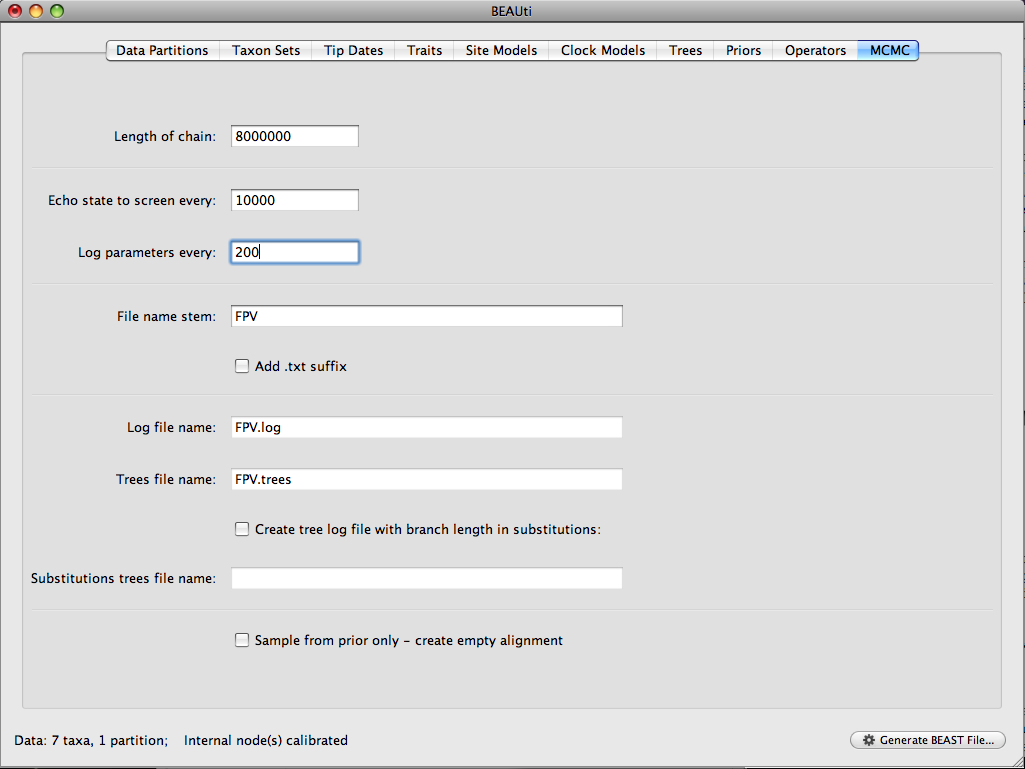
\includegraphics[scale=0.4]{figures1/BEAUti_MCMC}

\medskip{}

For this exercise we will set the screen log to 10000 and the file log to 200. The final two
options give the file names of the log files for the sampled parameters and
the trees. These will be set to a default based on the name of the
imported NEXUS file. 

\begin{itemize}
\item We suggest you add the suffix \texttt{.txt} to both of these (so,
\texttt{FPV.log.txt} and \texttt{FPV.trees.txt}) so that Windows recognizes
these as text files. 
\end{itemize}

\subsubsection*{Generating the BEAST XML file }

We are now ready to create the BEAST XML file. To do this,
either select the {\bf Generate BEAST File...} option from the File menu or click the similarly labelled button at the bottom of the
window. Save the file with an appropriate name
(we usually end the filename with \texttt{.xml}, i.e., \texttt{FPV.xml}).
We are now ready to run the file through BEAST. 

\subsection*{Running BEAST }

Now run BEAST and when it asks for an input file, provide your newly
created XML file as input. BEAST will then run until it has finished
reporting information to the screen. The actual results files are
save to the disk in the same location as your input file. The output to the screen will
look something like this: 

{\scriptsize   
\begin{verbatim}
                 
                 BEAST v1.5.1, 2002-2009
       Bayesian Evolutionary Analysis Sampling Trees
                 Designed and developed by
   Alexei J. Drummond, Andrew Rambaut and Marc A. Suchard
                              
               Department of Computer Science
                   University of Auckland
                  alexei@cs.auckland.ac.nz
                              
             Institute of Evolutionary Biology
                  University of Edinburgh
                     a.rambaut@ed.ac.uk
                              
              David Geffen School of Medicine
           University of California, Los Angeles
                     msuchard@ucla.edu
                              
                Downloads, Help & Resources:
                	http://beast.bio.ed.ac.uk/
                              
Source code distributed under the GNU Lesser General Public License:
           	http://code.google.com/p/beast-mcmc/
                              
                     BEAST developers:
	Alex Alekseyenko, Erik Bloomquist, Joseph Heled, Sebastian Hoehna, 
	Philippe Lemey, Gerton Lunter, Sidney Markowitz, Vladimir Minin, 
      	Michael Defoin Platel, Oliver Pybus, Walter Xie
                              
                         Thanks to:
    	Roald Forsberg, Beth Shapiro and Korbinian Strimmer

                  
Random number seed: 1251938914753


Parsing XML file: FPV.xml
  File encoding: MacRoman
Read alignment, ':alignment
  Sequences = 7
      Sites = 1434
   Datatype = nucleotide
Site patterns 'FPV.patterns' created from positions 1-1434 of alignment 'alignment'
  pattern count = 535
Using Yule prior on tree
Creating the tree model, 'treeModel'
  initial tree topology = ((((PumaPV1,SnowLeopardPV1),FelisPV1),(AsianLionPV1,LynxPV1)),
  (CanineOralPV,RacoonPV1))
  tree height = 419.51636733556074
Using discretized relaxed clock model.
  over sampling = 1
  parametric model = logNormalDistributionModel
   rate categories = 12
Creating state frequencies model: Using empirical frequencies from data = {0.25455, 0.24404, 
0.24965, 0.25175}
Creating HKY substitution model. Initial kappa = 1.0
Creating site model: 
  4 category discrete gamma with initial shape = 0.5
TreeLikelihood using native nucleotide likelihood core
  Ignoring ambiguities in tree likelihood.
  With 535 unique site patterns.
Branch rate model used: discretizedBranchRates
Creating swap operator for parameter branchRates.categories (weight=10.0)
WARNING: Element named statistic with idref=tmrca(Felis/Lynx/Puma) does not match stored object 
with same id and tag name tmrcaStatistic
WARNING: Element named statistic with idref=tmrca(Lion/Leopard) does not match stored object 
with same id and tag name tmrcaStatistic
Creating the MCMC chain:
  chainLength=8000000
  autoOptimize=true

Pre-burnin (80000 states)
0              25             50             75            100
|--------------|--------------|--------------|--------------|
*************************************************************

# BEAST v1.5.1, Build r2182
# Generated Thu Sep 03 12:48:53 NZST 2009 [seed=1251938914753]
state	Posterior   	Prior       	Likelihood  	Root Height 	Rate        
0	-8,121.8084 	-24.4568    	-8,097.3516 	11.7747     	3.90679E-2  	-
10000	-8,128.8259 	-27.1991    	-8,101.6269 	27.2727     	2.09442E-2  	0.32 hours/million states
20000	-8,127.6115 	-24.9343    	-8,102.6772 	21.5540     	2.79145E-2  	0.26 hours/million states
30000	-8,127.1922 	-28.3718    	-8,098.8204 	27.6143     	2.58108E-2  	0.24 hours/million states

780000	-8,126.7146 	-28.0645    	-8,098.6501 	31.0896     	2.06675E-2  	0.21 hours/million states
790000	-8,127.0498 	-26.1386    	-8,100.9112 	26.9619     	2.65692E-2  	0.21 hours/million states
800000	-8,127.1940 	-25.9037    	-8,101.2903 	25.2927     	2.35438E-2  	0.21 hours/million states

Operator analysis
Operator                                                  Pr(accept)  Performance suggestion
scale(kappa)                                      0.642   0.2428      good	
scale(alpha)                                      0.681   0.2623      good	
scale(ucld.mean)                                  0.725   0.2526      good	
scale(ucld.stdev)                                 0.332   0.3333      good	
subtreeSlide(treeModel)                           2.42    0.2668      good	
Narrow Exchange(treeModel)                                0.0656      good	
Wide Exchange(treeModel)                                  0.0115      good	
wilsonBalding(treeModel)                                  0.0027      low	
scale(treeModel.rootHeight)                       0.683   0.2438      good	
uniform(nodeHeights(treeModel))                           0.1793      good	
scale(yule.birthRate)                             0.235   0.3092      good	
up:ucld.mean down:nodeHeights(treeModel)          0.401   0.2339      slightly high	Try setting 
scaleFactor to about 0.401
swapOperator(branchRates.categories)                      0.5013      high	No suggestions
randomWalkInteger(branchRates.categories)                 0.8036      high	Try increasing windowSize 
to about 2.0
uniformInteger(branchRates.categories)                    0.6029      high	



10.098216666666668 minutes 
\end{verbatim}}

\subsection*{Analyzing the results}

Run the program called {\bf Tracer} to analyze the output of BEAST. When the main
window has opened, choose {\bf Import Trace File...} from the {\bf File} menu and select the file that
BEAST has created called \texttt{FPV.log.txt}.
You should now see a window like the following:

\medskip{}

\frame{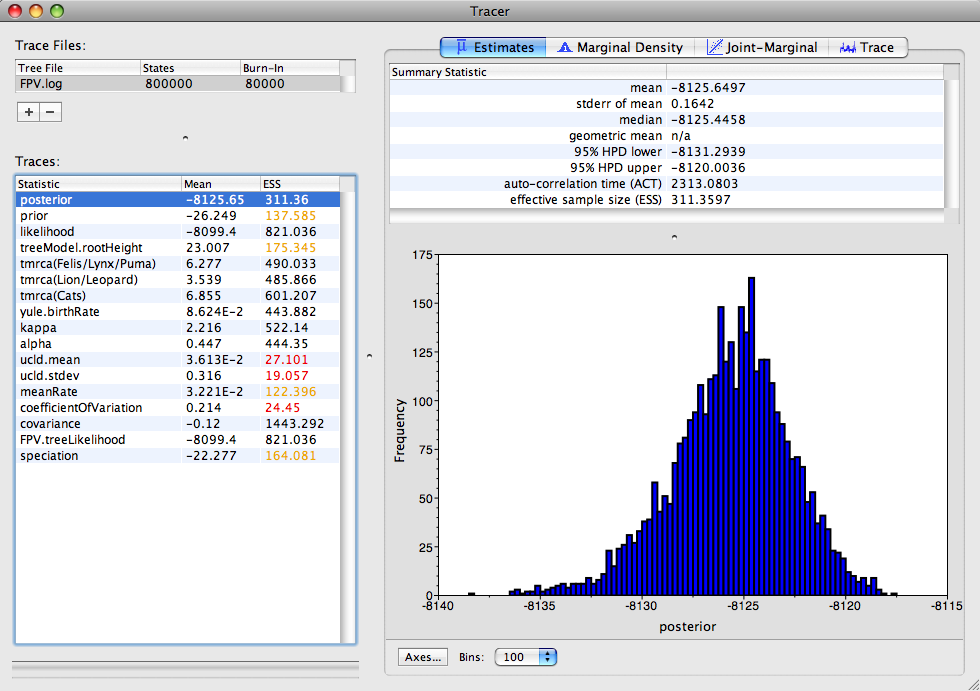
\includegraphics[scale=0.4]{figures1/Tracer1}}

\medskip{}

Remember that MCMC is a stochastic algorithm so the actual numbers will not be exactly the same.

On the left hand side is a list of the different quantities that BEAST has logged. 
There are traces for the posterior (this
is the log of the product of the tree likelihood and the prior probabilities), and the continuous parameters. Selecting a trace
on the left brings up analyses for this trace on the right hand side depending on tab that is selected. When first opened, the
`posterior' trace is selected and various statistics of this trace are shown under the Estimates tab.
In the top right of the window is a table of calculated statistics for the selected trace. 

Select \texttt{meanRate} to look at
the rate of evolution averaged over the whole tree. Tracer will plot a (marginal posterior) distribution for the selected parameter and also give you
statistics such as the mean and median. The 95\% HPD stands for {\it highest posterior density interval} and represents the most compact interval on the selected parameter that contains 95\% of the posterior probability. It can be thought of as a Bayesian analog to a confidence interval. 

\subsection*{Questions}
 \vspace{5 mm}

\textit{What is the rate of molecular evolution in FPV (include the HPD interval)?}

 \vspace{5 mm}
 \framebox(420,30){}
  \vspace{5 mm}


\textit{What sources of error does this estimate include?}
 
 \vspace{5 mm}
 \framebox(420,60){}
   \vspace{5 mm}
   
   The \texttt{coefficientOfVariation} statistic gives a summary of how much the rate of evolution varies from lineage to lineage (expressed as a proportion of the mean rate).
   
   \bigskip{}

\textit{Does the rate of evolution differ substantially amongst different lineages in the tree?}

 \vspace{5 mm}
 \framebox(420,60){}
   \vspace{5 mm}

Selecting the \texttt{treeModel.rootHeight} parameter gives the marginal posterior distribution of the age of the root of entire tree (i.e., the divergence between feline papillomavirus and canine oral papillomavirus).

   \bigskip{}

\textit{How old is the root of the tree (give the mean and the HPD range)?}

 \vspace{5 mm}
 \framebox(420,30){}
   \vspace{5 mm}

Select the \texttt{treeModel.rootHeight} parameter and the next three (hold shift whilst selecting). This will show a display of the
age of the root and the three MRCAs we specified in BEAUti. The two parameters that we used to calibrate the tree
(\texttt{tmrca(Felis/Lynx/Puma)} and \texttt{tmrca(Lion/Leopard)}) should have posterior distributions similar to the prior distributions
that we specified. If papilloma virus co-diverged with its host, then our estimate of \texttt{tmrca(Cats)}, should have a similar age to the origin
of the cats. The origin of the cats was estimated by Rector et al. (2007) as 10.78 My, +/-1.87.

\medskip{}

\frame{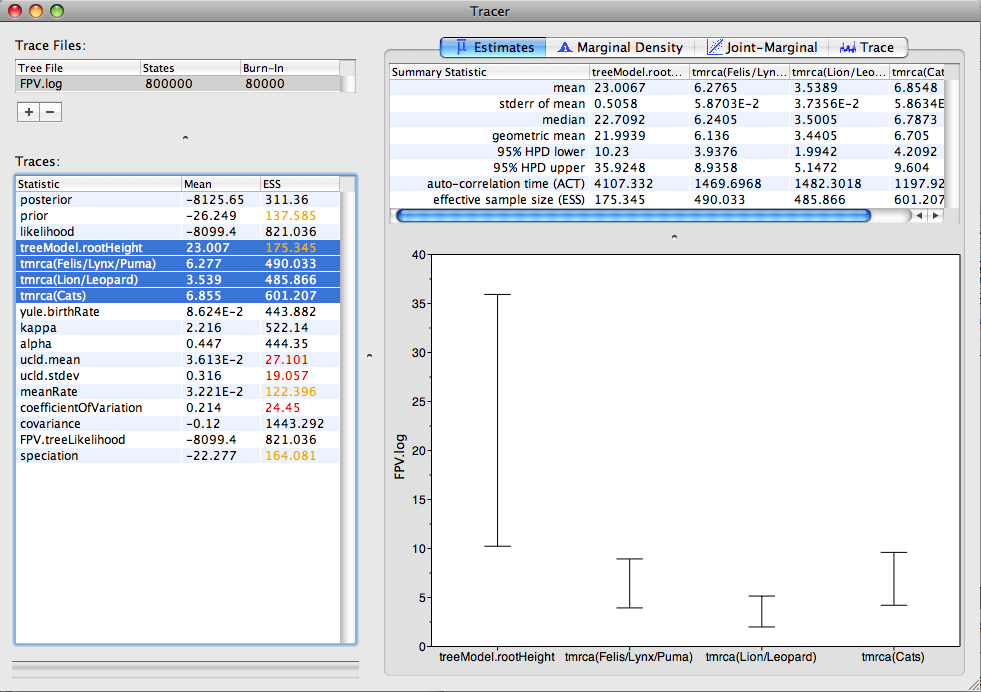
\includegraphics[scale=0.4]{figures1/Tracer_divergences}}

\medskip{}

If you switch the tab at the top of the window to {\bf Marginal Density} then you will get a plot of the marginal posterior densities of each of these date estimates overlayed:

\medskip{}

\frame{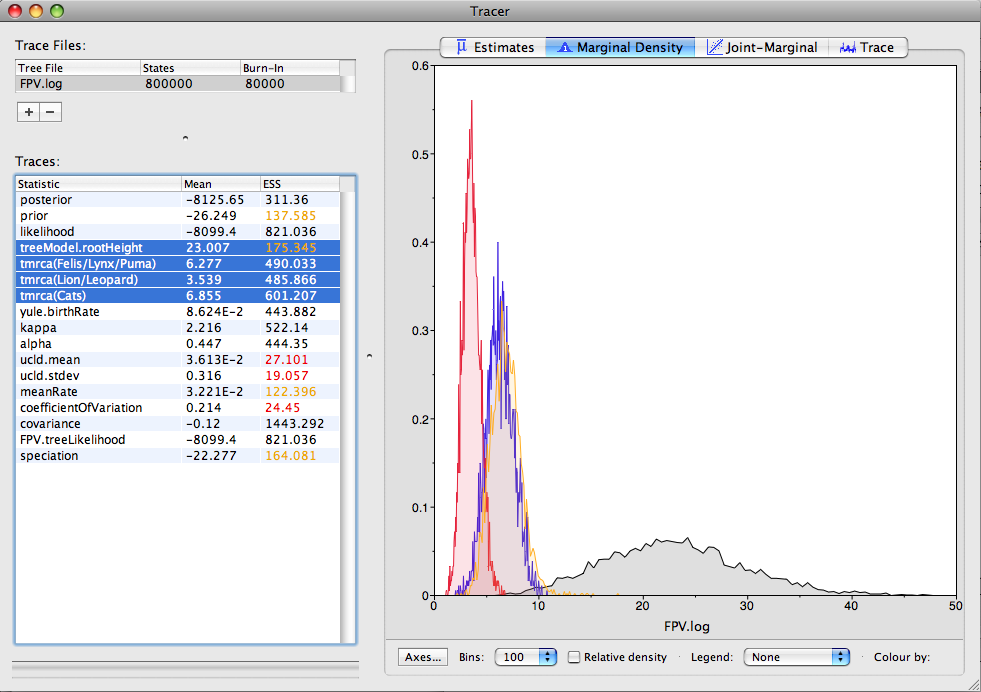
\includegraphics[scale=0.4]{figures1/Tracer_marginalDensity}}

\medskip{}

\subsection*{Obtaining an estimate of the phylogenetic tree}

BEAST also produces a sample of plausible trees along its sample of parameter estimates. 
These need to be summarized
using the program {\bf TreeAnnotator} (see Notes for details). This will take the set of trees and find the best
supported one. It will then annotate this summary tree with the mean ages of all the
nodes and the HPD ranges. It will also calculate the posterior clade probability for each
node. Run the TreeAnnotator program and set it up to look like this:

\medskip{}

\frame{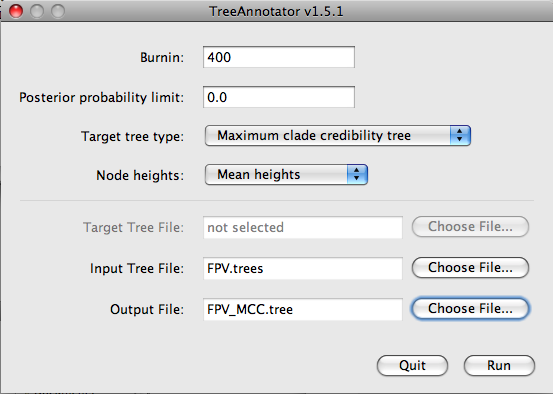
\includegraphics[scale=0.5]{figures1/TreeAnnotator1}}

\medskip{}

The burnin is the number of trees to remove from the start of the sample. Unlike {\bf Tracer} which specifies the number of
steps as a burnin, in {\bf TreeAnnotator} you need to specify the actual number of trees. For this run, you specified a chain
length of 800,000 steps sampling every 200 steps. Thus the trees file will contain 4000 trees and so to specify a 10\% burnin
use the value 400.

The {\bf Posterior probability limit} option specifies a limit such that if a node is found at less than this frequency in the sample
of trees (i.e., has a posterior probability less than this limit), it will not be annotated. The default of 0.5 means that only nodes
seen in the majority of trees will be annotated. Set this to zero to annotate all nodes.

For {\bf Target tree type} you can either choose a specific tree from a file or ask TreeAnnotator to find a tree in your sample.
The default option, {\bf Maximum clade credibility tree}, finds the tree with the highest product of the posterior probability of
all its nodes.

Choose {\bf Mean heights} for node heights. This sets the heights (ages) of each node in the tree to the mean height across the
entire sample of trees for that clade.

For the input file, select the trees file that BEAST created (by default this will be called \texttt{FPV.trees}) and select a file for the
output (here we called it \texttt{FPV\_MCC.tree}).

Now press Run and wait for the program to finish.

\subsection*{Viewing the Tree}
Finally, we can look at the tree in another program called {\bf FigTree}. Run this program, and open
the \texttt{FPV\_MCC.tree} file by using the Open command in the File menu. The tree should appear.
You can now try selecting some of the options in the control panel on the left. Try selecting
{\bf Node Bars} to get node age error bars. Also turn on {\bf Branch Labels} and select {\bf posterior} to get
it to display the posterior probability for each node. Under {\bf Appearance} you can also tell FigTree
to colour the branches by the rate.
You should end up with something like this:

\medskip{}

\frame{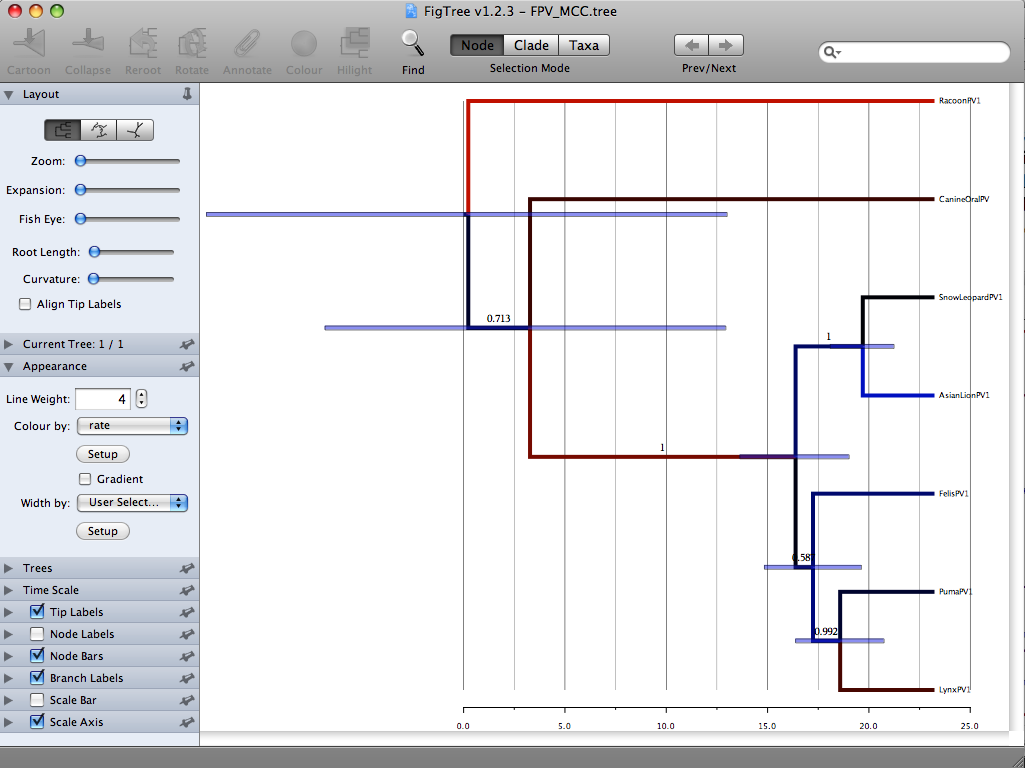
\includegraphics[scale=0.4]{figures1/FigTree}}

\medskip{}

\textit{Which branch has the fastest rate of evolution and what is the estimated rate?}

 \vspace{5 mm}
 \framebox(420,30){}
  \vspace{5 mm}


\textit{Which branch has the slowest rate of evolution and what is the estimated rate?}
 
 \vspace{5 mm}
 \framebox(420,30){}
   \vspace{5 mm}

\textit{Are these two rate estimates significantly different? How would you answer this question?}
 
 \vspace{5 mm}
 \framebox(420,60){}
   \vspace{5 mm}


\subsection*{Comparing your results to the prior}

Using BEAUti, set up the same analysis but under the MCMC options, select the {\bf Sample from prior only} option:

\medskip{}

\frame{
\includegraphics[scale=0.7]{figures1/SamplePriorOnly}}

\medskip{}

This will allow you to visualize the full prior distribution in the absence of your sequence data. Summarize the trees from the full prior
distribution and compare the summary to the posterior summary tree.

\pagebreak

%%%%%%%%%%%%%%%%%%%%%%%%%%%%%%%%%%%%%%%%%%%%%
%%%
%%% EXERCISE 2 - TIME-STAMPED DATA
%%%
%%%%%%%%%%%%%%%%%%%%%%%%%%%%%%%%%%%%%%%%%%%%%

\section*{Exercise 2: Time-stamped data}

This exercise estimates the rate of evolution from a set of virus sequences which have been isolated at different points in time (heterochronous or time-stamped data). The data are 35 sequences from the G (attachment protein) gene of human respiratory
syncytial virus subgroup A (RSVA) from various parts of the world with isolation dates ranging from 1956-2002 (Zlateva,
Lemey, Vandamme \& Van Ranst, ``Molecular evolution and circulation patterns of human respiratory syncytial virus subgroup
a: positively selected sites in the attachment g glycoprotein.'' {\it J Virol} 2004, {\bf 78}: 4675-4683. 2004).

The aim is to obtain estimates for :

\begin{itemize}
\item the rate of molecular evolution
\item the date of the most recent common ancestor
\item the phylogenetic relationships with appropriate measures of statistical support.
\end{itemize}

\subsection*{The NEXUS alignment}
Select the file called \texttt{RSVA.nex}. This file contains an alignment of 35 sequences from the G gene of RSVA virus, 629 nucleotides in length.

Open this file in BEAUti. By default all the taxa are assumed to have a date of zero (i.e. the sequences are assumed to be sampled at the same time).
In this case, the RSVA sequences have been sampled at various dates going back to the 1950s. The actual year of sampling
is given in the name of each taxon and we could simply edit the value in the Date column of the table to reflect these.
However, if the taxa names contain the calibration information, then a convenient way to specify the dates of the sequences
in BEAUti is to use the ``Guess Dates'' button at the top of the {\bf Tip Dates} panel. Clicking this will make a dialog box appear:

\medskip{}

\frame{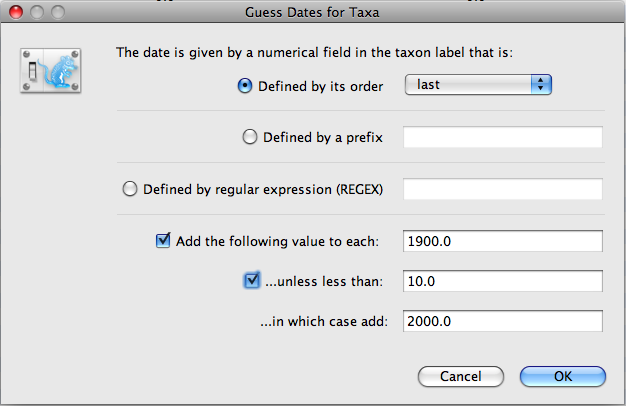
\includegraphics[scale=0.5]{figures2/GuessDates}}

\medskip{}

Select the options as shown in the figure above. For more information about the {\bf Guess Dates} facility see the Notes.

\subsection*{Setting the substitution model}
The next thing to do is to set the substitution model in the {\bf Site Models} tab. For this exercise, we will select the {\bf 3 partitions: codon positions 1, 2 \& 3} option so that each codon position has its own rate of
evolution. For more information about linking/unlinking model parameters across codon positions see the Notes.

\medskip{}

\frame{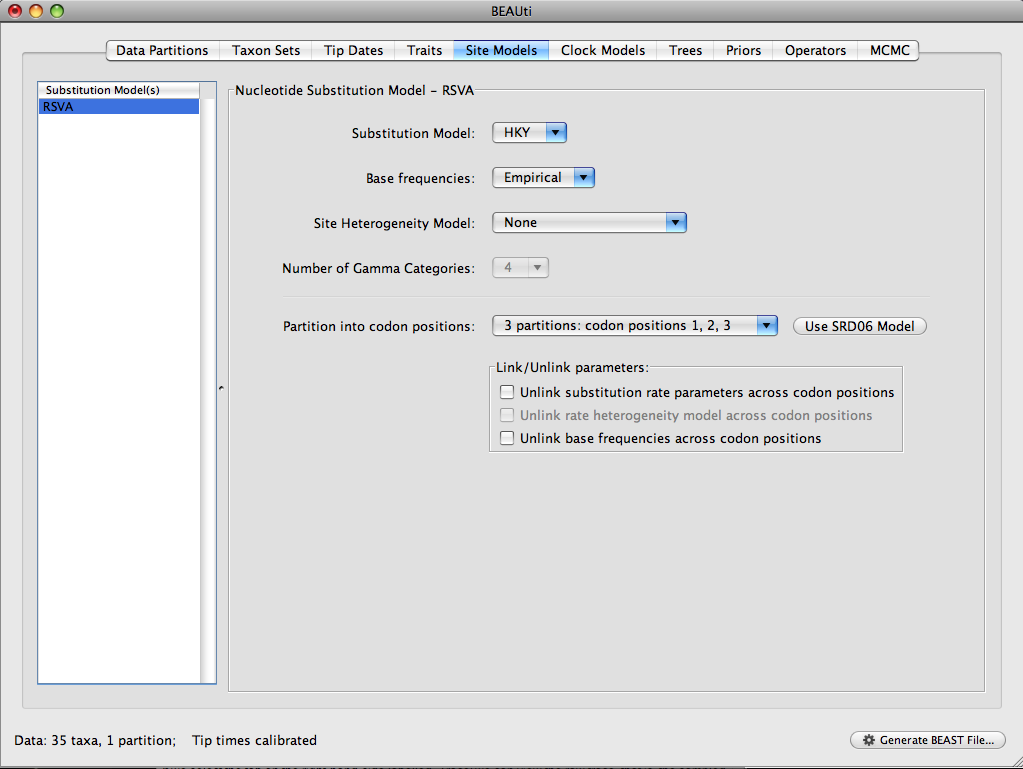
\includegraphics[scale=0.4]{figures2/BEAUTi_Subst_Model}}

\medskip{}

\subsection*{Setting the MCMC options}

For this dataset let's initially set the chain length to 150,000 as this will run 
reasonably quickly on most modern computers. Set the sampling frequencies 
to 1000 and 150 respectively.

\subsection*{Running BEAST}

Generate a BEAST XML named \texttt{RSVA.xml} and run it in BEAST.

\subsection*{Analysing the BEAST output}

Note that the effective sample sizes (ESSs) for many of the logged quantities are small (ESSs less than 100 will be highlighted in red by Tracer).
This is not good. A low ESS means that the trace contained a lot of correlated samples and thus may not represent the
posterior distribution well. In the bottom right of the window is a frequency plot of the samples which is expected given the
low ESSs is extremely rough.

If we select the tab on the right-hand-side labelled `Trace' we can view the raw trace, that is, the sampled values against the step in the MCMC chain.

\medskip{}

\frame{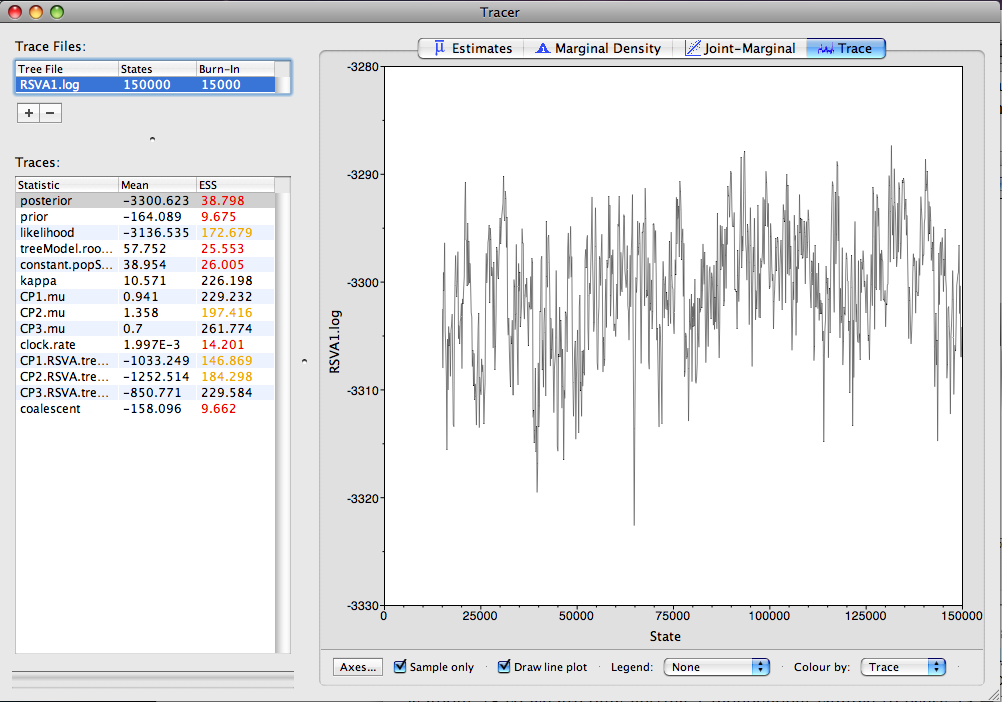
\includegraphics[scale=0.40]{figures2/Tracer1}}

\medskip{}

Here you can see how the samples are correlated. There are 1000 samples in the trace (we ran the MCMC for 150,000
steps sampling every 150) but adjacent samples often tend to have similar values. The ESS for the age of the
root (treeModel.rootHeight is about 78 so we are only getting 1 independent sample to every $13=1000/78$ actual samples). With such a short run it may also be the case that the default burn-in of 10\% of the chain length is inadequate. Not excluding enough of the start of the chain as burn-in will render estimates of ESS unreliable.

The simple response to this situation is that we need to run the chain for longer. Given the lowest ESS (for the prior) is 31, it
would suggest that we have to run it at least 7 times longer to get reasonable ESSs that are $>$200. However it would be better to aim
higher so lets go for a chain length of 2,000,000. Go back to the {\bf MCMC} options section in BEAUti, and create a new BEAST
XML file with a longer chain length. Now run BEAST and load the new log file into Tracer (you can leave the old one loaded
for comparison). Click on the Trace tab and look at the raw trace plot.

\medskip{}

\frame{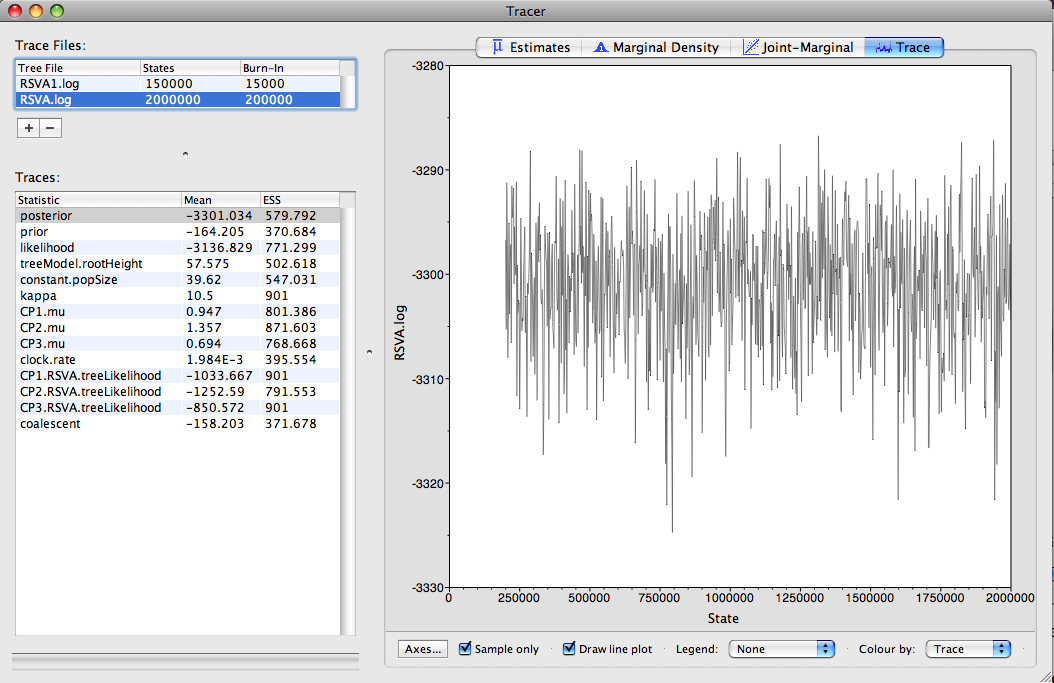
\includegraphics[scale=0.40]{figures2/Tracer2}}

\medskip{}

Again we have chosen options that produce 1000 samples and with an ESS of about 600 there is still auto-correlation
between the samples but 600 effectively independent samples will now provide a good estimate of the posterior distribution.
There are no obvious trends in the plot which would suggest that the MCMC has not yet converged, and there are no significant long range 
fluctuations in the trace which would suggest poor mixing.

As we are happy with the mixing we can now move on to one of the parameters of interest:
substitution rate. Select \texttt{clock.rate} in the left-hand table. This is the average substitution rate across all sites in the
alignment. Now choose the density plot by selecting the tab labeled Density. This shows a plot of the posterior probability
density of this parameter. You should see a plot similar to this:

\medskip{}

\frame{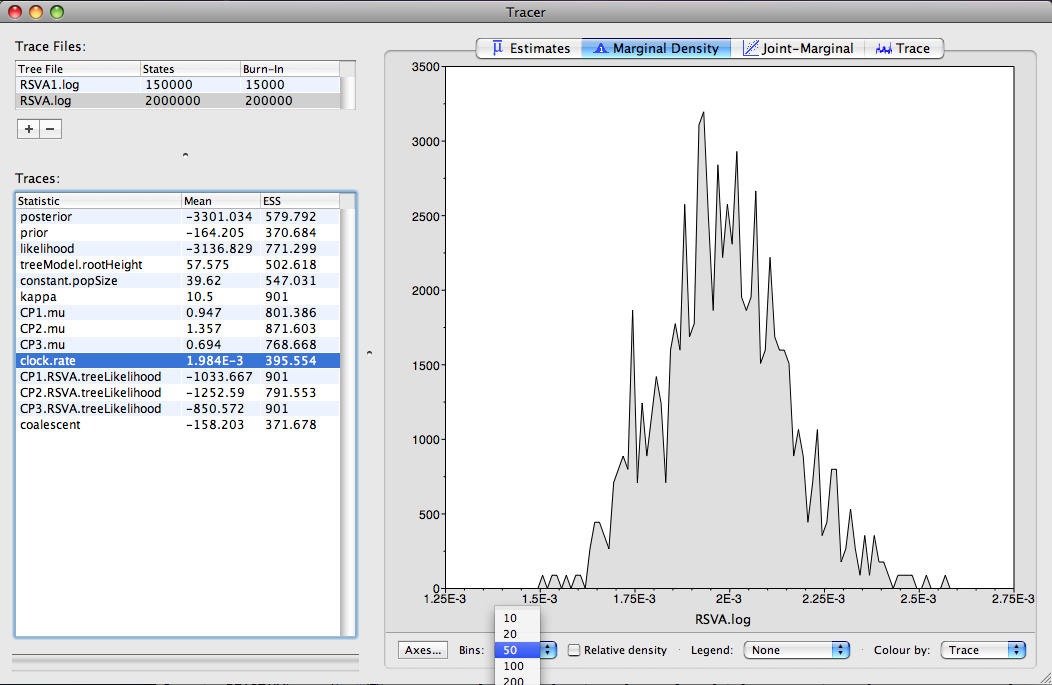
\includegraphics[scale=0.40]{figures2/Tracer_density}}

\medskip{}

As you can see the posterior probability density is roughly bell-shaped. There is some sampling noise which would be
reduced if we ran the chain for longer or sampled more often but we already have a good estimate of the mean and HPD interval. You can overlay
the density plots of multiple traces in order to compare them (it is up to the user to determine whether they are comparable on the the same axis or not). Select the relative substitution rates for all three codon positions in the table to the left (labelled
\texttt{CP1.mu}, \texttt{CP2.mu} and \texttt{CP3.mu}). You will now see the posterior probability densities for the relative
substitution rate at all three codon positions overlaid:

\medskip{}

\frame{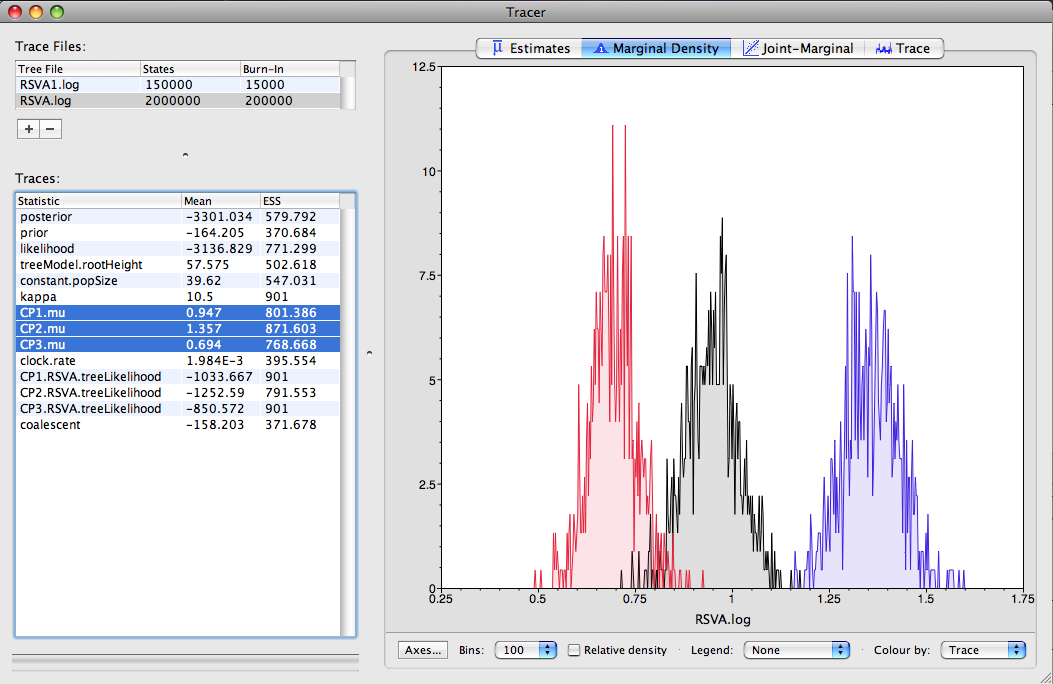
\includegraphics[scale=0.40]{figures2/Tracer_relativeRates}}

\medskip{}

\textit{In what year did the common ancestor of all RSVA viruses sampled live? What is the 95\% HPD?}
 
 \vspace{5 mm}
 \framebox(420,30){}
   \vspace{5 mm}

\subsection*{Summarizing the trees}

Use TreeAnnotator to summarize the tree:

\medskip{}

\frame{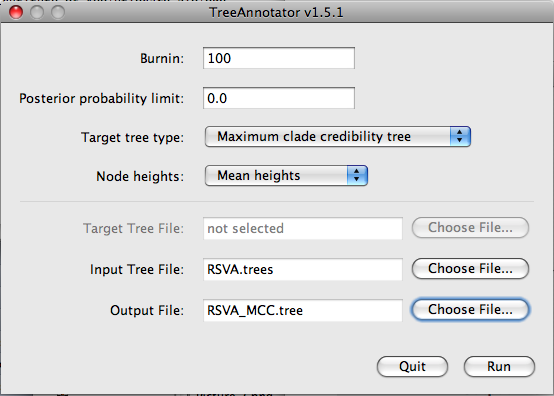
\includegraphics[scale=0.5]{figures2/TreeAnnotator}}

\medskip{}

And view the results in Figtree:

\medskip{}

\frame{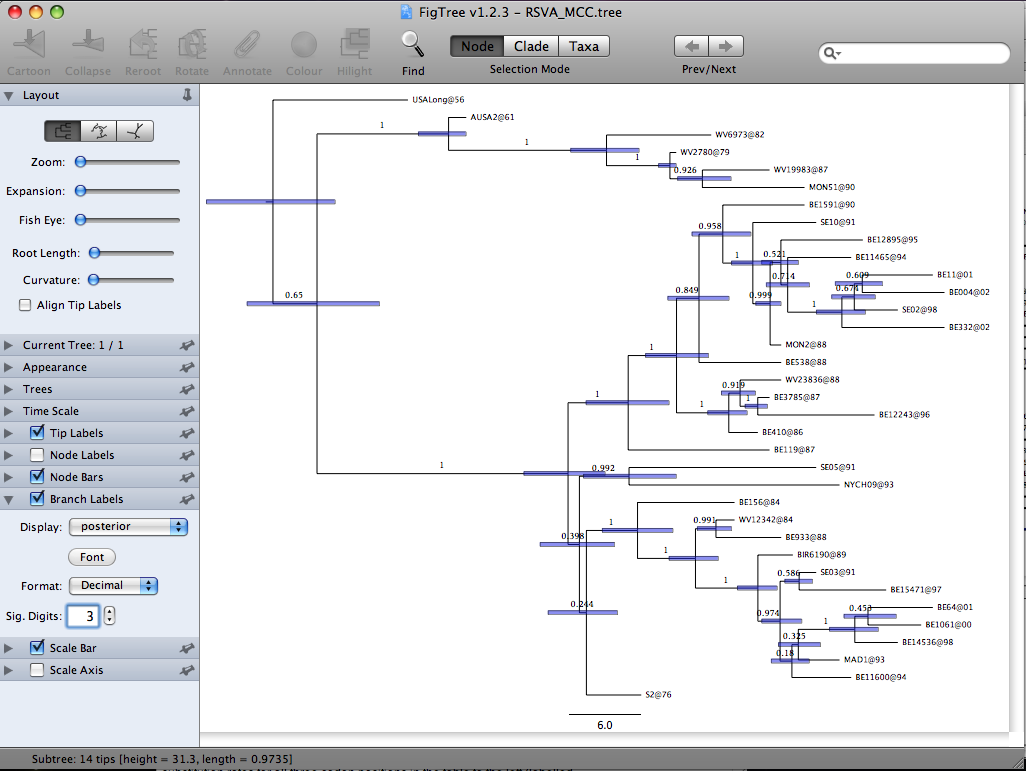
\includegraphics[scale=0.4]{figures2/Figtree}}

\pagebreak

%%%%%%%%%%%%%%%%%%%%%%%%%%%%%%%%%%%%%%%%%%%%%
%%%
%%% EXERCISE 3 - BAYESIAN SKYLINE PLOT
%%%
%%%%%%%%%%%%%%%%%%%%%%%%%%%%%%%%%%%%%%%%%%%%%

\section*{Exercise 3: Bayesian skyline plot}

In this exercise we will investigate the population history of the the H5N1 influenza epidemic, by using the Bayesian Skyline Plot (BSP), which estimates changes in effective population size through time. The data are 21 H5N1 strain Influenza A sequences sampled between 1997 and 2005 from Southeast Asia; including viruses from birds, pigs and humans.

\subsubsection*{The NEXUS alignment}

Open the file called \texttt{Flu.nex} in BEAUti. This file contains an alignment of 21 sequences from the Influenza A virus, 1698
nucleotides in length. 

By default all the taxa are assumed to have a date of zero (i.e. the sequences are assumed to be sampled at the same time).
In this case, the Influenza sequences have been sampled at various dates going back to 1997. The actual year of sampling
is given in the name of each taxon and we could simply edit the value in the Date column of the table to reflect these.
However we can also use the ``Guess Dates'' facility. In the {\bf Guess Dates} dialog box select \texttt{last} in the drop down and click the ``OK'' button. The dates will appear in the appropriate
column of the main window. You can then check these and edit them manually if required. 

\subsection*{Setting the substitution model}

For this exercise, select the {\bf 3 partitions: codon positions 1, 2 \& 3} option so that each codon position has its own rate of
evolution.

\subsection*{Setting the tree prior}

In the {\bf Trees} panel select {\bf Coalescent: Bayesian Skyline} for the tree prior. We will also reduce the number of steps to 5 from the default of 10 because we only have 21 sequences and we don't want to over-parameterize the model.

\medskip{}

\frame{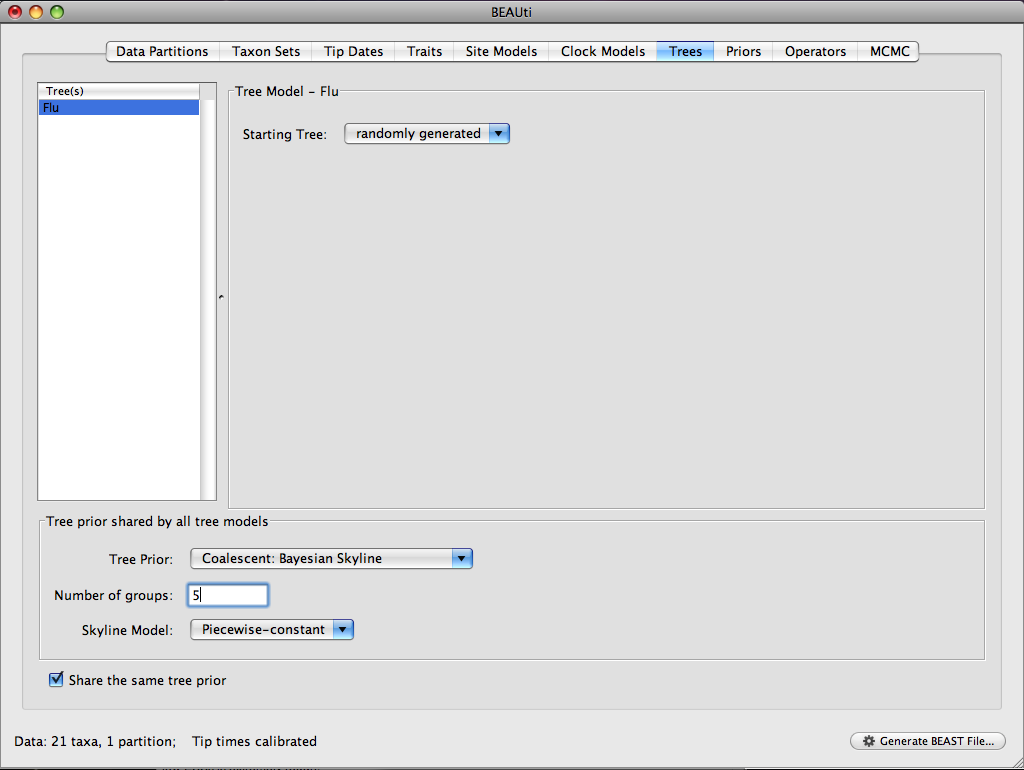
\includegraphics[scale=0.4]{figures3/BEAUTi_Tree}}

\medskip{}

\subsection*{Setting the MCMC options}

For this dataset let's initially set the chain length to 3,000,000. This will take 10-30 minutes on a fast computer. Set the two sampling frequencies to 3000 and 1000 respectively.

\subsection*{Running BEAST}

Generate a BEAST XML named \texttt{Flu.xml} and run it in BEAST.

\subsection*{Analysing the BEAST output}

You can overlay the density plots of multiple logged quantities in order to compare them (it is up to the user to determine whether they are comparable on the the same axis or not). Select the relative substitution rates for all three codon positions in the table to the left (labelled
\texttt{CP1.mu}, \texttt{CP2.mu} and \texttt{CP3.mu}). You will now see the posterior probability densities for the relative
substitution rate at all three codon positions overlaid:

\medskip{}

\frame{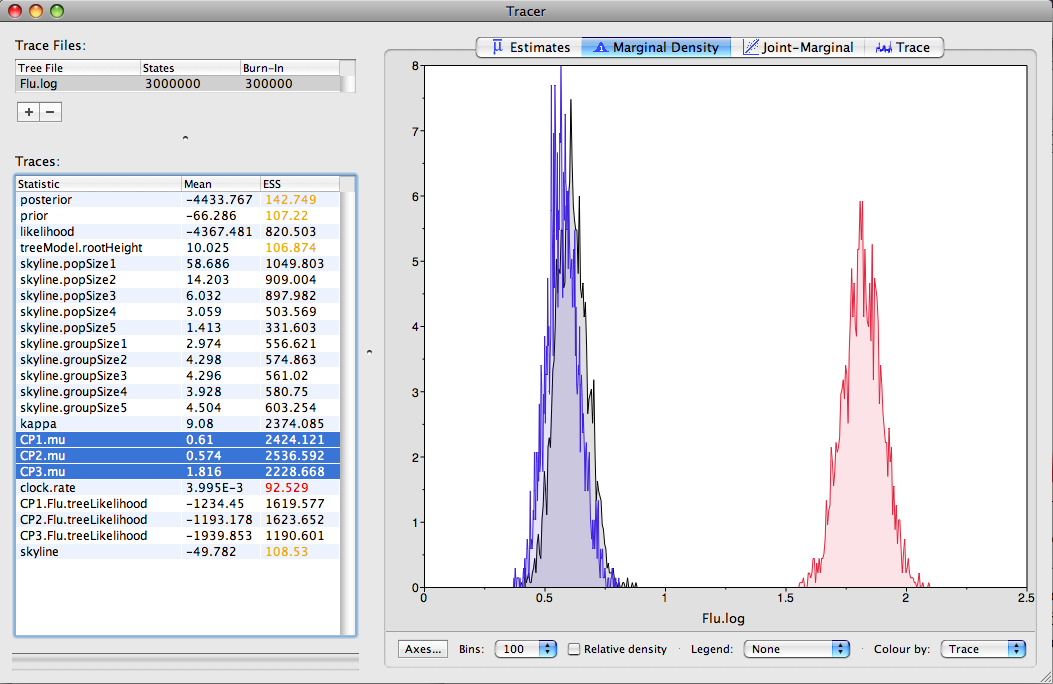
\includegraphics[scale=0.40]{figures3/Tracer_relativeRates}}

\medskip{}

This plot clearly shows that the evolution of these sequences is dominated by purifying selection as the 3rd codon position (known as the wobble position) has a much higher rate of evolution (about 3 times faster) than either of the other codon positions.

\subsection*{Constructing the Bayesian skyline plot}

To construct the BSP simply select {\bf Bayesian Skyline Reconstruction...} from the {\bf Analysis} menu. Select the appropriate trees log file (e.g. \texttt{Flu.trees}) that corresponds to the parameter  log file loaded in Tracer. The remaining default values in the dialog box will be fine, so click OK. After the trees file is processed the BSP should appear in a new window:

\medskip{}

\frame{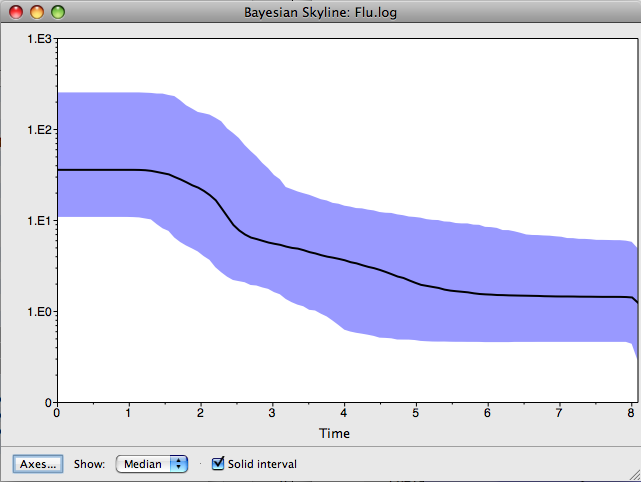
\includegraphics[scale=0.60]{figures3/Tracer_BSP}}

\medskip{}

\textit{By what amount did the effective population size of H5N1 Influenza grow from 1997 to 2005 according to the BSP?}
 
 \vspace{5 mm}
 \framebox(420,30){}
   \vspace{5 mm}

\textit{What are the underlying assumptions of the BSP? Are the violated by this data set?}
 
 \vspace{5 mm}
 \framebox(420,90){}
   \vspace{5 mm}


\subsection*{Summarizing the trees}

Summarize the trees file using TreeAnnotator:

\medskip{}

\frame{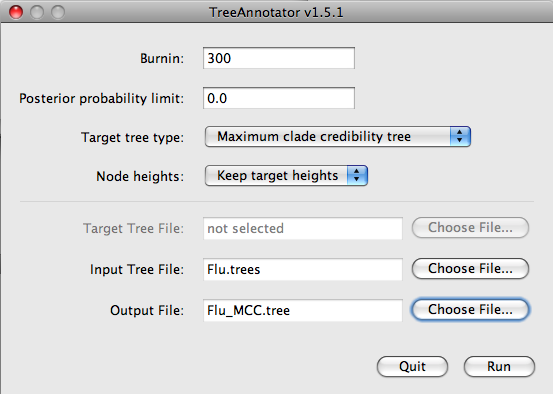
\includegraphics[scale=0.5]{figures3/TreeAnnotator}}

\medskip{}

And view it in FigTree:

\medskip{}

\frame{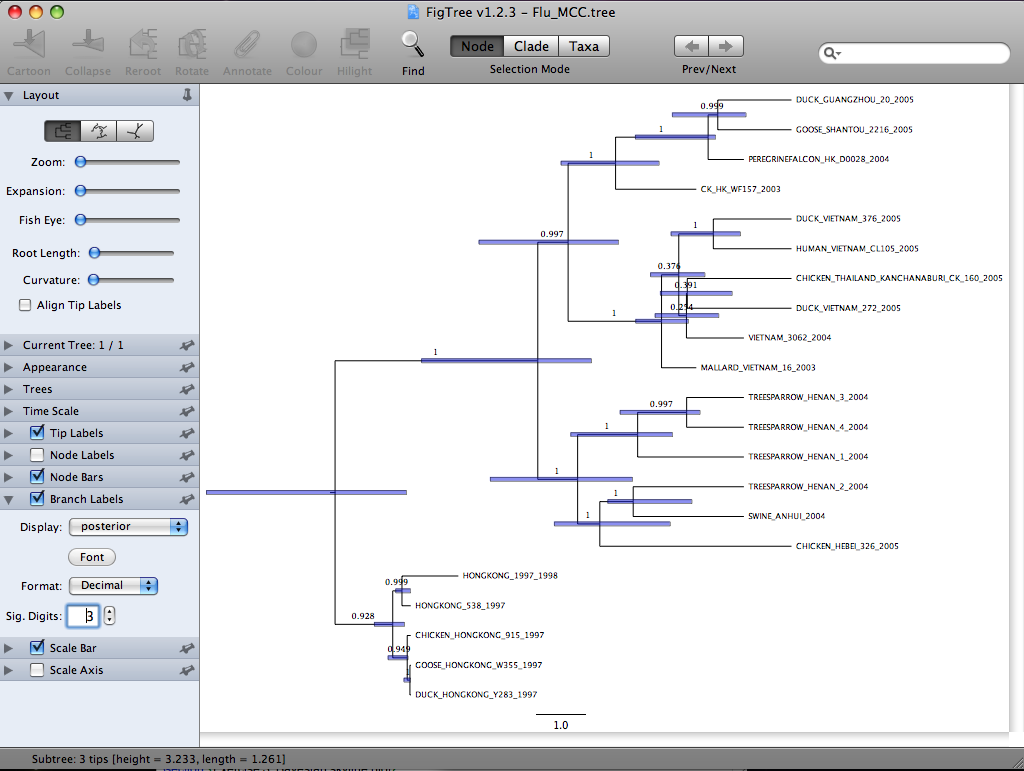
\includegraphics[scale=0.4]{figures3/Figtree}}

\medskip{}

\subsection*{Conclusion and Resources}
This practical only scratches the surface of the analyses that are possible to undertake using BEAST. It has hopefully provided
a relatively gentle introduction to the fundamental steps that will be common to all BEAST analyses and provide a basis for
more challenging investigations. BEAST is an ongoing development project with new models and techniques being added
on a regular basis. The BEAST website provides details of the mailing list that is used to announce new features and to
discuss the use of the package. The website also contains a list of tutorials and recipes to answer particular evolutionary
questions using BEAST as well as a description of the XML input format, common questions and error messages.

\begin{itemize}
\item The BEAST website: \texttt{http://beast.bio.ed.ac.uk/}
\item Tutorials: \texttt{http://beast.bio.ed.ac.uk/Tutorials/}
\item Frequently asked questions: \texttt{http://beast.bio.ed.ac.uk/FAQ/}
\end{itemize}

\section*{Notes}

This section has some extra details about aspects of some of the programs.

\subsection*{Guess Dates}

This operation attempts to guess what the dates are from information contained within the taxon names. It works by trying to
find a numerical field within each name. If the taxon names contain more than one numerical field (such as the RSVA
sequences in Exercise 2) then you can specify how to find the one that corresponds to the date of sampling. You can either
specify the order that the date field comes (e.g., first, last or various positions in between) or specify a prefix (some
characters that come immediately before the date field in each name). For the RSVA sequences you can select `last' from
the drop-down menu for the order or use the prefix option and specify `\_' (underscore) as the prefix.

In this dialog box, you can also get BEAUti to add a fixed value to each guessed date. In this case the value ``1900'' has
been added to turn the dates from 2 digit years to 4 digit. Any dates in the taxon names given as ``00'' would thus become
``1900''. Some of the sequences in the example file actually have dates after the year 2000 so selecting the will option would
convert them correctly, adding 2000 to any date less than 09. When you press OK the dates will appear in the appropriate
column of the main window. You can then check these and edit them manually as required. At the top of the window you
can set the units that the dates are given in (years, months, days) and whether they are specified relative to a point in the
past (as would be the case for years such as 1984) or backwards in time from the present (as in the case of radiocarbon
ages).

\subsection*{Operators}
Each parameter in the model has one or more ``operators'' (these are variously called moves and proposals by other MCMC
software packages such as MrBayes and LAMARC). The operators specify how the parameters change as the MCMC runs.
The operators tab in BEAUti has a table that lists the parameters, their operators and the tuning settings for these operators.
In the first column are the parameter names. These will be called things like \texttt{kappa} which means the HKY model's
kappa parameter (the transition-transversion bias). The next column has the type of operators that are acting on each
parameter. For example, the scale operator scales the parameter up or down by a proportion, the random walk operator
adds or subtracts an amount to the parameter and the uniform operator simply picks a new value uniformly within a range.
Some parameters relate to the tree or to the divergence times of the nodes of the tree and these have special operators.

The next column, labelled {\bf Tuning}, gives a tuning setting to the operator. Some operators don't have any tuning settings so
have {\bf n/a} under this column. The tuning parameter will determine how large a move each operator will make which will affect
how often that change is accepted by the MCMC which will affect the efficency of the analysis. For most operators (like
random walk and subtree slide operators) a larger tuning parameter means larger moves. However for the scale operator a
tuning parameter value closer to 0.0 means bigger moves. At the top of the window is an option called {\bf Auto Optimize}
which, when selected, will automatically adjust the tuning setting as the MCMC runs to try to achieve maximum efficiency. At
the end of the run a table of the operators, their performance and the final values of these tuning settings will be written to
standard output. These can then be used to set the starting tuning settings in order to minimize the amount of time taken to
reach optimum performance in subsequent runs.

The next column, labelled {\bf Weight}, specifies how often each operator is applied relative to the others. Some parameters
tend to be sampled very efficiently - an example is the kappa parameter - these parameters can have their operators downweighted
so that they are not changed as often (this may mean weighting other operators up since the weights must be
integers).

\subsection*{Codon position models}

\begin{itemize}
\item Selecting the {\bf Partition into codon positions} option assumes that the data are aligned as codons. This option will then
estimate a separate rate of substitution for each codon position, or for 1+2 versus 3, depending on the setting.
Estimating rates and dates from time-sample sequences � a hands-on practical
3
\item Selecting the {\bf Unlink substitution model across codon positions} will specify that BEAST should estimate a separate
transition-transversion ratio or general time reversible rate matrix for each codon position.
\item Selecting the {\bf Unlink rate heterogeneity model across codon positions} will specify that BEAST should estimate set
of rate heterogeneity parameters (gamma shape parameter and/or proportion of invariant sites) for each codon position.
\item If there are no dates for the sequences (they are contemporaneous) then you can specify a fixed mean substitution rate
obtained from another source. Setting this to 1.0 will result in the ages of the nodes of the tree being estimated in units of
substitutions per site (i.e. the normal units of branch lengths in popular packages such as MrBayes).
\end{itemize}

\subsection*{Tracer statistics}

The statistics reported in Tracer for each logged quantity are:

\begin{itemize}
\item Mean - The mean value of the samples (excluding the burn-in).
\item Stdev - The standard error of the mean. This takes into account the effective sample size so a small ESS will give a large
standard error.
\item Median - The median value of the samples (excluding the burn-in).
95\% HPD Lower - The lower bound of the highest posterior density (HPD) interval. The HPD is the shortest interval that
contains 95\% of the sampled values.
\item 95\% HPD Upper - The upper bound of the highest posterior density (HPD) interval.
\item Auto-Correlation Time (ACT) - The average number of states in the MCMC chain that two samples have to be separated
by for them to be uncorrelated (i.e. independent samples from the posterior). The ACT is estimated from the samples in the
trace (excluding the burn-in).
\item Effective Sample Size (ESS) - The effective sample size (ESS) is the number of independent samples that the trace is
equivalent to. This is calculated as the chain length (excluding the burn-in) divided by the ACT.
\end{itemize}

\subsection*{TreeAnnotator}

The sampled trees in BEAST are written to a separate file called the `trees' file. This file is a
standard NEXUS format file. As such it can easily be loaded into other software in order to examine the trees it contains. One
possibility is to load the trees into a program such as PAUP* and construct a consensus tree in a similar manner to
summarizing a set of bootstrap trees. In this case, the support values reported for the resolved nodes in the consensus tree
will be the posterior probability of those clades.

TreeAnnotator is a software program distributed with BEAST that can summarize the tree file. 
It takes a single `target' tree and annotates it with the summarized information from the entire sample of trees.
The summarized information includes the average node ages (along with the HPD intervals), the posterior support and the
average rate of evolution on each branch (for models where this can vary). The program calculates these values for each
node or clade observed in the specified `target' tree. The options in TreeAnnotator are detailed below:

\begin{itemize}
\item {\bf Burnin} - This is the number of trees in the input file that should be excluded from the summarization. This value is given
as the number of trees rather than the number of steps in the MCMC chain. Thus for the example above, with a chain of
1,000,000 steps, sampling every 1000 steps, there are 1000 trees in the file. To obtain a 10\% burnin, set this value to
100.
\item {\bf Posterior probability limit} - This is the minimum posterior probability for a node in order for TreeAnnotator to store the
annoted information. The default is 0.5 so only nodes with this posterior probability or greater will have information
summarized (the equivalent to the nodes in a majority-rule consensus tree). Set this value to 0.0 to summarize all nodes in
the target tree.
\item {\bf Target tree type} - This has two options ``Maximum clade credibility'' or ``User target tree''. For the latter option, a
NEXUS tree file can be specified as the Target Tree File, below. For the former option, TreeAnnotator will examine every
tree in the Input Tree File and select the tree that has the highest sum of the posterior probabilities of all its nodes.
\item {\bf Node heights} - This option specifies what node heights (times) should be used for the output tree. If the ``Keep target
heights'' is selected, then the node heights will be the same as the target tree. The other two options give node heights
as an average (Mean or Median) over the sample of trees.
\item {\bf Target Tree File} - If the ``User target tree'' option is selected then you can use ``Choose File...'' to select a NEXUS file
containing the target tree.
\item I{\bf nput Tree File} - Use the ``Choose File...'' button to select an input trees file. This will be the trees file produced by
BEAST.
\item {\bf Output File} - Select a name for the output tree file.
\end{itemize}

Once you have selected all the options, above, press the ``Run'' button. 

\end{document}
